%  Register_Design.tex
%  Document created by seblovett on seblovett-Ubuntu
%  Date created: Thu 17 Apr 2014 14:59:55 BST
%  <+Last Edited: Sun 11 May 2014 15:16:13 BST by seblovett on seblovett-Ubuntu +>

\section{Register Block}

%Design of whole module, including circuit diagram
The register block contains eight general purpose registers. 
No dummy register is implemented in the register block. 
The module has three address inputs, two read addresses and one write address. 
There are two read outputs, which output the stored data, and a data input to be written.% \todo[inline, color=green]{MW: This does not make sense to me}
Reads are asynchronous and must always be driven. 
Writes are synchronous and must implement a write enable signal. 

%Use of hierarchy / blocks - i.e. bit sliced, decoder
To optimise the design for space, the module is broken down into a bit slice and a decoder. 
The whole block is made up of sixteen slices and one decoder. 

\subsection{Bit Slice Design}

The bit slice consists of eight load enable registers. 
Two tristate buffers are used per register onto different buses for the two read data outputs. 
The registers are selected by one hot coding and as such will result in the output bus always being driven. 
The write enables are also controlled using one hot coding. 
However, all signals are allowed to be off if no register is to be written to.
The circuit diagram for the bit slice is seen in Figure~\ref{fig:reg:slice}.

\begin{figure}
\centering
\includegraphics[angle=90,height=\textheight]{../../eagle/regBlock/regBlock_slice.png}
\caption{Circuit diagram for the register block slice.}
\label{fig:reg:slice}
\end{figure}



\begin{table}
\caption{Decoder Logic Functions}
\label{tab:reg:decoder}
\centering
\begin{tabular}{cc}
Register Number & Logic Select Function \\
0		&		$!( Rs0 | Rs1 | Rs2 )$ \\
1		&		$ !( Rs1 | Rs2 ) \& Rs0$	\\
2		&		$!( Rs2 | Rs0 ) \& Rs1$\\
3		&		$! ( ! ( Rs0 \& Rs1 ) | Rs2 )$	\\
4		&		$!( Rs0 | Rs1 ) \& Rs2$	\\
5		&		$! ( ! ( Rs0 \& Rs2 ) | Rs1 )$	\\
6		&		$! ( ! ( Rs1 \& Rs2 ) | Rs0 )$	\\
7		&		$Rs0 \& Rs1 \& Rs2$	\\
\end{tabular}

\end{table}

The read decoder is based around a 3-8 decoder. 
For each 3 bit input, one and only one output should be high. 
The logic functions used are summarised in Table~\ref{tab:reg:decoder}.
The bit sliced circuit diagram is shown in Figure~\ref{fig:reg:decoder}.
This illustrates only one of the decoders needed since the second is identical.
However, the write decoder must also use a write enable signal.
This is done by using the same logic functions shown in Table~\ref{tab:reg:decoder}, but the resulting signals are then \texttt{AND}ed with the register write enable signal. 
%\todo[inline, color=green]{MW: Ive re-worded this a bit}
%\todo[inline, color=green]{MW: what do you mean by write enable function?}

\begin{figure}
\centering
%\missingfigure{Decoder circuit diagram}
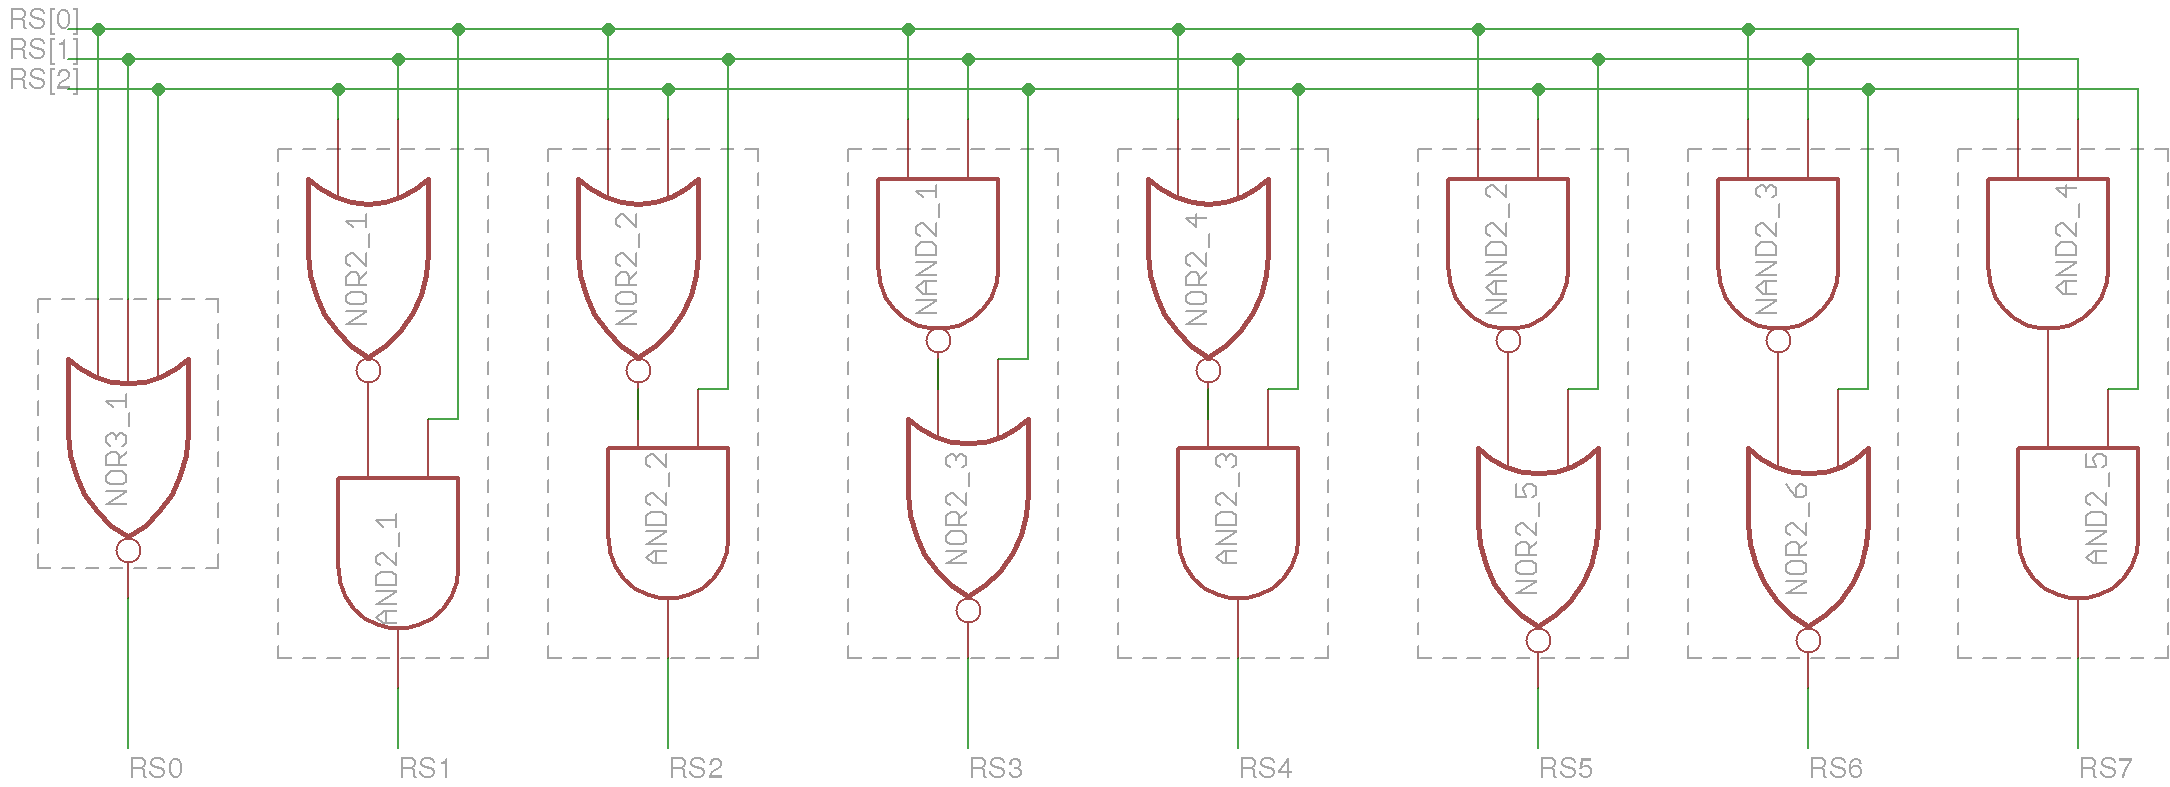
\includegraphics[width=\textwidth]{../../eagle/regBlock/regBlock_decoder.png}
\caption{Circuit diagram for the register decoder.}
\label{fig:reg:decoder}
\end{figure}
%Design of block,

%Layout in silicon
The layout in silicon consisted of an array of slices. 
All I/Os for the slice are then in the same position and all global signals from the decoder are propagated through the slice.
The use of tristate buffers reduces the wiring needed in the design. 
The decoder was designed to fit above the block of general purpose registers. 
All three decoders were distributed in the implementation and spaced to reduce the size of the wiring channel.
\todo[inline, color=green]{MW: which buffers? HSL: what? }
